\documentclass{article}
\usepackage[utf8]{inputenc}
\usepackage{graphicx}

\author{Bijan Varjavand}
\title{Lab Write-up}

\begin{document}

\maketitle

Our buckling load equation is
$$P = \frac{E\pi ^3D^3}{4L^2}$$
$$E = \frac{4PL^2}{\pi ^3D^4}$$

We can confirm the powers by plotting the data on log scales.

\begin{figure}[h]
	\centering
	\begin{minipage}{0.5\textwidth}
		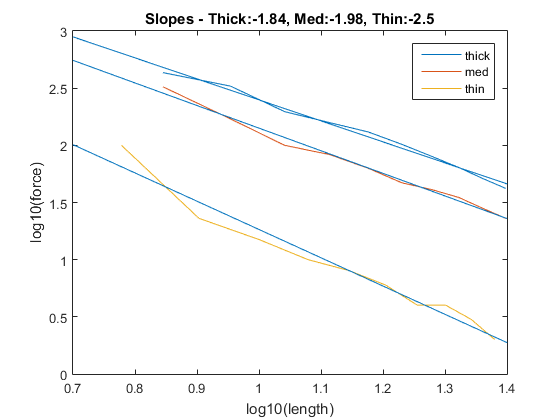
\includegraphics[scale=0.3]{Lab1f1.png}
	\end{minipage}%
	\begin{minipage}{0.5\textwidth}
		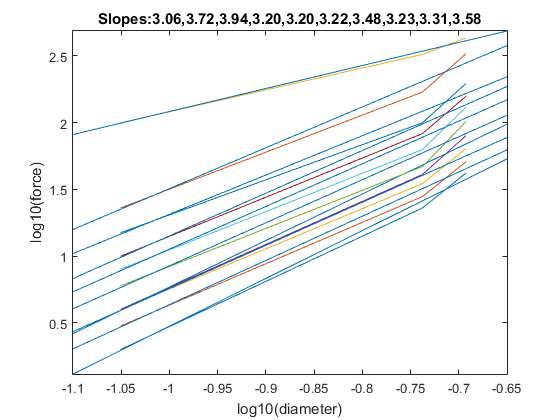
\includegraphics[scale=0.3]{Lab1f3.png}
	\end{minipage}
	\caption{Averages for the slopes = -3.6 and 1.5}
\end{figure}

The ruler we used had an error of $\pm$ 0.5mm, and the scale had an error of $\pm$ 0.5g.

Calculating standard deviation of the length, radius, and pressure:
$$\sigma = \sqrt{\frac{1}{N}\sum_{i=i}^N{(x_i-\mu )^2}}$$
$$\sigma _{length} = 5.8624,\ \sigma _{diameter} = 0.4539,\ \sigma _{force} = 109.6030$$

Error propagation given by
$$\delta q = \sqrt{(\delta x^2)+(\delta z)^2 + (\delta \omega )^2}$$
$$\frac{\delta E}{E} = \frac{4}{\pi ^3}\sqrt{(\frac{2\delta L}{L})^2 + (\frac{-4\delta R}{R})^2 + (\frac{\delta P}{P})^2}$$
$$\frac{\delta E}{E}$$

$$Mean(E) = 5.4534 \frac{g}{cm*s^2} = 54.534 \frac{kg}{m*s^2}$$

\end{document}